\chapter{Giải pháp và phương án thực hiện}
\label{Chapter3}

\emph{Chương này sẽ trình bày, mô tả chi tiết về các nghiên cứu sẽ thực hiện để giải quyết bài toán xây dựng chatbot chỉ đường, bao gồm việc trích xuất ý định và thực thể}

\section{Giải pháp xây dựng ứng dụng}
Dưới đây là sơ đồ xây dựng ứng dụng chatbot:
\begin{figure}[htp]
    \centering
    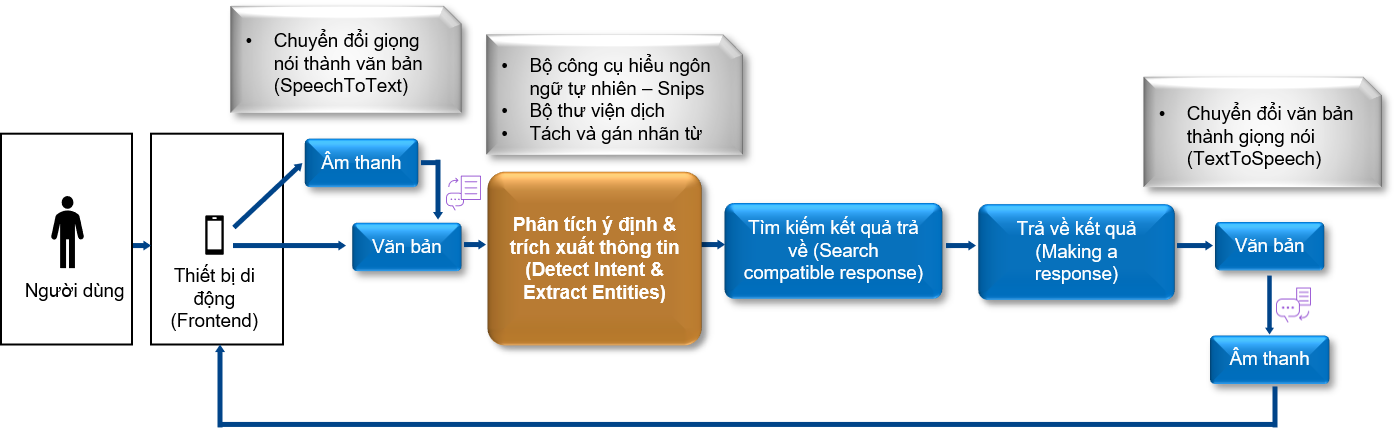
\includegraphics[width=10cm]{images/Structure-description.png}
    \caption{Sơ đồ của hệ thống chỉ đường}
    \label{fig:sodohethongchiduong}

\end{figure}

Sơ đồ này thể hiện các bước thực hiện để xây dựng ứng dụng chatbot từ dữ liêụ đầu vào đến kết quả nhận được. Các bước thực hiện được triển khai như sau:
\begin{itemize}
    \item[--] Bước 1: Khi người dùng sử dụng ứng dụng di động gửi một câu truy vấn bằng audio thì ứng dụng di động sẽ chuyển giọng nói đó thành văn bản (speech to text).
    \item[--] Bước 2: Văn bản đó được gửi tới NLU engine để trích xuất ý định và các thực thể.
    \item[--] Bước 3: Dựa trên ý định và thực thể nhận được, hệ thống sẽ tìm kiếm câu trả lời tương ứng và trả về cho người dùng bằng text và audio (text to speech để chuyển văn bản thành giọng nói).
\end{itemize}
Trong phạm vi đề tài, nhóm sẽ xây dựng thành phần xác định ý định,trích xuất dữ liệu và tìm kiếm kết quả trả lời câu hỏi sẽ sử dụng API của Google Map.

Nhóm chúng em quyết định sử dụng Snips \ac{nlu} cho việc xác định intent vì:
\begin{itemize}
    \item[--] Miễn phí vì nó là opensource
    \item[--] Gọn nhẹ và dễ dàng sử dụng vì có cộng đồng lớn
    \item[--] Hiệu suất cao.
\end{itemize}

Trong hình dưới đây(Xem hình Bảng so sánh \ref{fig:benchmarks}), điểm F1 của cả phân loại ý định và trích xuất slot đã được tính toán cho một số nhà cung cấp NLU và được tính trung bình trên ba bộ dữ liệu Lights dataset\footnote{Xem thêm về Lights dataset tại đây:\url{https://github.com/snipsco/snips-nlu/blob/master/sample_datasets/lights_dataset.json}}, Beverage dataset\footnote{Xem thêm về Beverage dataset tại đây:\url{https://github.com/snipsco/snips-nlu/blob/master/sample_datasets/beverage_dataset.json}}, Flights dataset\footnote{Xem thêm về Flights dataset tại đây:\url{https://github.com/snipsco/snips-nlu/blob/master/sample_datasets/flights_dataset.json}}.

\begin{figure}[htp]
    \centering
    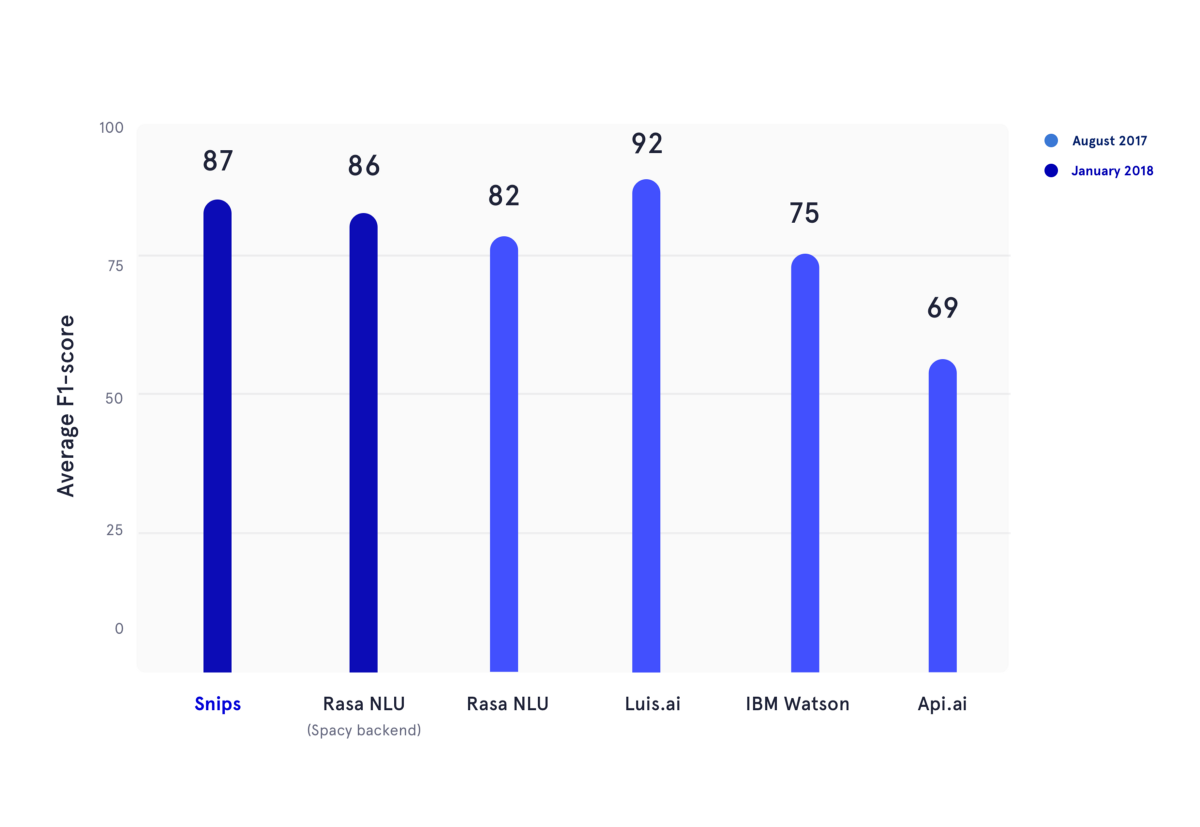
\includegraphics[width=10cm]{images/benchmarks.png}
    \caption{Bảng so sánh}
    \label{fig:benchmarks}
\end{figure}

Snips NLU là công cụ giúp hiểu ngôn ngữ tự nhiên mạnh mẽ, nhưng hiện tại chưa hỗ trợ tiếng Việt, mục tiêu của chúng em là xây dựng một chatbot bằng tiếng Việt. Vì thế, để có thể sử dụng được Snips-nlu để trích xuất ý định và thực thể, chúng em tiến hành thực hiện các bước sau đây:
\begin{itemize}
    \item[--] Bước 1: Tạo một bộ dữ liệu bằng tiếng Việt với các câu nói về chủ đề đường đi.
    \item[--] Bước 2: Chuyển hoá dữ liệu tiếng Việt sang tiếng Anh.
    \item[--] Bước 3: Dùng dữ liệu tiếng Anh được dịch sang để huấn luyện cho mô hình.
    \item[--] Bước 4: Chuyển hoá văn bản bằng tiếng Việt nhận vào sang tiếng Anh.
    \item[--] Bước 5: Đưa câu nói bằng tiếng Anh vào mô hình để trích xuất ý định và các thực thể.
\end{itemize}

Về mặt dữ liệu:
\begin{itemize}
    \item[--] Định dạng bộ dữ liệu huấn luyện là ở dạng json.
\end{itemize}